\documentclass[a4paper,12pt]{article}
\usepackage{fullpage}
\usepackage[T1]{fontenc}
\usepackage{amsmath}
\usepackage{amssymb}
\usepackage[utf8]{inputenc}
\usepackage{color}
\usepackage{authblk}
\usepackage{todonotes}
\usepackage{caption}
\usepackage{url}
\usepackage{float}
\usepackage{sectsty}
\usepackage{pdfpages}
\usepackage[section]{placeins}
\DeclareCaptionFont{white}{\color{white}}
\DeclareCaptionFormat{listing}{\colorbox{gray}{\parbox{\textwidth}{#1#2#3}}}
\captionsetup[lstlisting]{format=listing,labelfont=white,textfont=white}

\usepackage{setspace}
\usepackage[toc,page]{appendix}
\usepackage{framed}
\usepackage{geometry}

\usepackage{alltt}
\usepackage{subfig}

% Change section fonts
\allsectionsfont{\sffamily}

% For code box
\usepackage{xcolor}
\usepackage{listings}
\usepackage{caption}
\DeclareCaptionFont{white}{\color{white}}
\DeclareCaptionFormat{listing}{%
  \parbox{\textwidth}{\colorbox{gray}{\parbox{\textwidth}{#1#2#3}}\vskip-4pt}}
  \captionsetup[lstlisting]{format=listing,labelfont=white,textfont=white}
  \lstset{frame=lrb,xleftmargin=\fboxsep,xrightmargin=-\fboxsep}
% End code box

\usepackage{cite}

% General parameters, for ALL pages:
\renewcommand{\topfraction}{0.9}	% max fraction of floats at top
\renewcommand{\bottomfraction}{0.8}	% max fraction of floats at bottom
% Parameters for TEXT pages (not float pages):
\setcounter{topnumber}{2}
\setcounter{bottomnumber}{2}
\setcounter{totalnumber}{4} % 2 may work better
\setcounter{dbltopnumber}{2} % for 2-column pages

\addtolength{\topmargin}{0.5in}

\usepackage{fancyvrb}

\usepackage{tikz} \usetikzlibrary{trees}
\usepackage{hyperref} % should always be the last package

% useful colours (use sparingly!):
\newcommand{\blue}[1]{{\color{blue}#1}}
\newcommand{\green}[1]{{\color{green}#1}}
\newcommand{\red}[1]{{\color{red}#1}}

% useful wrappers for algorithmic/Python notation:
\newcommand{\length}[1]{\text{len}(#1)}
\newcommand{\twodots}{\mathinner{\ldotp\ldotp}} % taken from clrscode3e.sty
\newcommand{\Oh}[1]{\mathcal{O}\left(#1\right)}

% useful (wrappers for) math symbols:
\newcommand{\Cardinality}[1]{\left\lvert#1\right\rvert}
\newcommand{\Ceiling}[1]{\left\lceil#1\right\rceil}
\newcommand{\Floor}[1]{\left\lfloor#1\right\rfloor}
\newcommand{\Iff}{\Leftrightarrow}
\newcommand{\Implies}{\Rightarrow}
\newcommand{\Intersect}{\cap}
\newcommand{\Sequence}[1]{\left[#1\right]}
\newcommand{\Set}[1]{\left\{#1\right\}}
\newcommand{\SetComp}[2]{\Set{#1\SuchThat#2}}
\newcommand{\SuchThat}{\mid}
\newcommand{\Tuple}[1]{\langle#1\rangle}
\newcommand{\Union}{\cup}
\usetikzlibrary{positioning,shapes,shadows,arrows}
\providecommand{\keywords}[1]{\textbf{\textit{Keywords: }} #1}

\title{\textbf{Designing a Virtual Security Layer for Cloud Content}}
\author{Lukas Klingsbo}

\begin{document}

\maketitle
%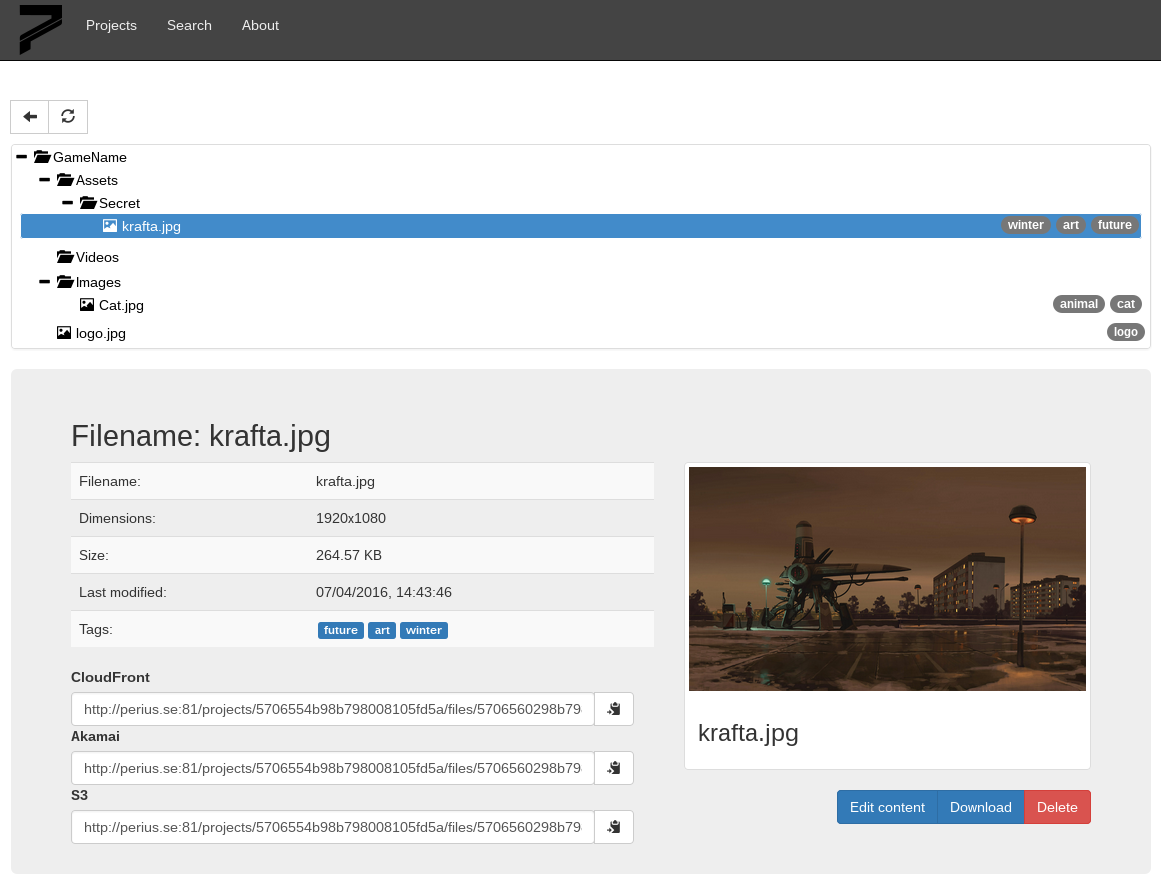
\includepdf[pages={1}]{front.pdf}
%\thispagestyle{empty}
%\newpage\null\thispagestyle{empty}\newpage

\pagenumbering{roman}
\setcounter{page}{2}

%\includepdf[pages={1}]{abstract.pdf}
\begin{abstract}
    TODO: Abstract

\keywords{}
\end{abstract}

\newpage\null\thispagestyle{empty}\newpage

\setcounter{tocdepth}{3}
\tableofcontents

\clearpage
\pagenumbering{arabic}
\setcounter{page}{1}
\section{Introduction}
Developing larger projects containing static content usually involves using a Content Distribution Network 
to be able to scale to a large user base. The commercial Content Distribution Networks are usually fairly easy to use, 
the content that is to be used in a project is usually simply uploaded and then directly available to the public. 
For secret content this can be a problem and that is what this thesis is about. This work examines ways of enforcing 
access control on content and groups of content in the form of views. A system was developed to make the underlying 
theory work in practice. 

\newpage
\section{Related Terminology}
\subsection{Technologies}
\subsubsection{React}
React is a JavaScript library for building user interfaces. React uses both its own virtual DOM and the browser's, 
this makes it able to efficiently update dynamic web pages after a change of state through comparing the old virtual 
DOM with the resulting virtual DOM after the state change and then only update the browser's DOM according to the 
difference between the virtual DOMs~\cite{REACT}.

\subsubsection{Flux}


\subsubsection{Scala}
Scala is a multi-paradigm programming language. It most commonly runs on the JVM and compared to Java it supports 
most functional programming features at the same time as it supports object oriented programming~\cite{SCALA}.

\subsubsection{REST}
Over http? WebSockets? 
\subsubsection{TODO: Insert persistent storage here}
    TODO: Write down related terminology, if any
\subsection{Abbreviations}

\subsubsection{CDN}
Content Distribution Network - Replicates content to several servers, usually spread out geographically. Once a 
request is made, the network serves content from the server closest to the requester.

\section{Related Work}
\subsection{Copy-on-Write}
This work relies heavily on the Copy-on-Write principle which was founded and used in the Mach kernel~\cite{COPYONWRITE}. 
Today Copy-on-Write is used in everything from file systems~\cite{BTRFS} to desktop compositors~\cite{COMPOSITOR}.

Its principle is that when processes share data in between each other, the data is not copied until one of the processes 
does changes to it. This is an optimisation as the processes does not have to send all of the related data that is in memory, 
rather they only have to send pointers to the data. After many Copy-on-Write's a complex structure can be built up, 
but it is possible to solve that structure~\cite{COPYONWRITE2}.

\section{Background}
\subsection{About Uprise}
Uprise is a company based in Uppsala, Sweden. 

\subsection{The current system}
Maybe write about battlebinary?  

\subsection{Problem description}
Having
  
Battle Binary

What is needed
* Security layers
* Views
* Virtual file structure
* Versioning of content
* Multi project support
* Auth and audit logs
* Users

\section{Model}
\subsection{Entities}
%\subsubsection*{View} for not having section numbers
\begin{figure}[htp] \centering{
    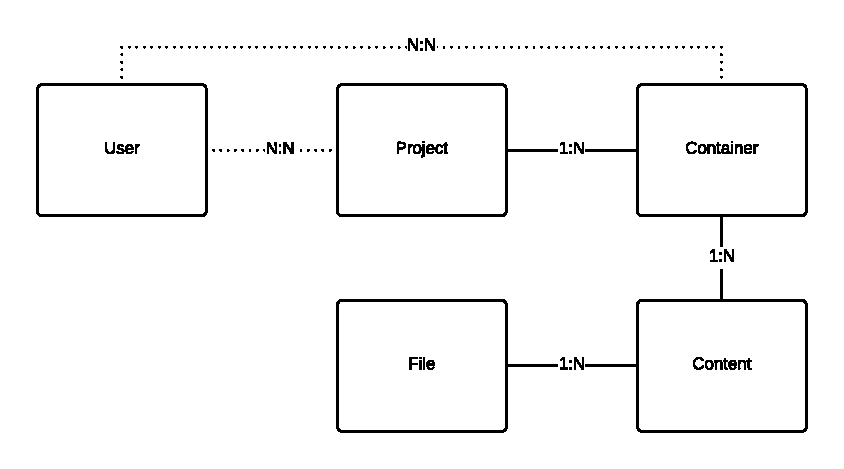
\includegraphics[scale=0.8]{relation.pdf}}
    \caption{Entity Relationships}
    \label{fig:relation}
\end{figure}

\subsubsection{View}
A view is a group of files which can be changed independently of the view's parent.
A view can have subviews which are either automatically dependant on its parent and 
updated when the parent is updated or optionally updated or forked from its parent 
once their content diverge.

\subsubsection{Project}
A project is just a name for the view which is a root of a tree of views.
The system can contain several projects and their trees are completely disjoint.

\subsubsection{File}
A file refers to an actual physical file in the file system.

\subsubsection{Content}
Content is an asset contained in a view, it is a virtual file.
It could be described as a link between the view and the real file. 
It can be for example an image, video or binary blob combined with meta-data.

\subsubsection{User}
A user is the structure that handles people who has been granted access to the system.
Access to the system is handled by a separate service, like LDAP.

\section{Copy-on-Write}

\section{Methods for determining\\implementation details}
This chapter introduces the different methods used to determine how the new system should be implemented, 
which DBMS it should use and how the estimation of long term scaling was done.

\section{Security of the system}
\subsection{Authorization}
\subsection{Audit logs}


\section{Resulting system}
\subsection{REST Endpoints}
For the frontend to communicate with the backend REST is used, the following endpoints were configured:

\begin{itemize}
  \item projects
      \subitem GET - list all projects
      \subitem POST - create new project
  \item projects/\{id\}
      \subitem GET - get specific project
      \subitem PUT - update existing project
      \subitem DELETE - delete existing project
  \item projects/\{id\}/content
      \subitem GET - list all content in a specific project
      \subitem POST - create new content in a specific project 
  \item projects/\{id\}/content/\{id\}
      \subitem GET - get specific content in a specific project
      \subitem PUT - update existing content in a specific project
      \subitem DELETE - delete existing content in a specific project

  \item projects/\{id\}/views
      \subitem GET - list all views in a specific project
      \subitem POST - create new view in a specific project 
  \item projects/\{id\}/views/\{id\}
      \subitem GET - get specific view in a specific project
      \subitem PUT - update existing view
      \subitem DELETE - delete existing view
  \item projects/\{id\}/views/\{id\}/content
      \subitem GET - list all content in a specific view
      \subitem POST - create new content in a specific view 
  \item projects/\{id\}/views/\{id\}/content/\{id\}
      \subitem GET - get specific content in a specific view
      \subitem PUT - update existing content in a specific view
      \subitem DELETE - delete existing content in a specific view
\end{itemize}

\subsection{Scalability}

\section{Discussion}

\section{Summary}
\subsection{Conclusions}

\subsection{Future work}

Stuff to write about:
Modular design, every piece should be interchangable
LDAP - why it was used as standard AUTH


\newpage
\bibliographystyle{ieeetr}
\bibliography{references}

\end{document}
